\documentclass[a4paper]{article}
\usepackage{tikz}
\usetikzlibrary{automata, positioning, arrows}
\usepackage[document]{ragged2e}

\tikzset{
->, % makes the edges directed
>=stealth', % makes the arrow heads bold
node distance=3cm, % specifies the minimum distance between two nodes. Change if necessary.
every state/.style={thick, fill=gray!10}, % sets the properties for each 'state' node
initial text=$ $, % sets the text that appears on the start arrow
}

\begin{document}



\section{Heading on Level 1 (section)}
This is an example of how to use the tikz libraries in LaTeX to draw state machine diagrams, DFAs, NFAs and Turing Machines.

\bigskip


\begin{figure}[ht] % 'ht' tells LaTeX to place the figure 'here' or at the top of the page
\centering % centers the figure

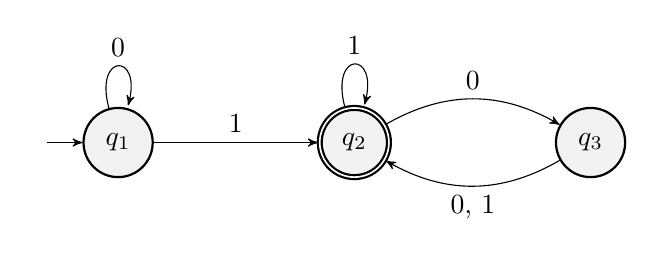
\begin{tikzpicture}
\node[state, initial] (q1) {$q_1$};
\node[state, accepting, right of=q1] (q2) {$q_2$};
\node[state, right of=q2] (q3) {$q_3$};
\draw (q1) edge[loop above] node{0} (q1)
(q1) edge[above] node{1} (q2)
(q2) edge[loop above] node{1} (q2)
(q2) edge[bend left, above] node{0} (q3)
(q3) edge[bend left, below] node{0, 1} (q2);
\end{tikzpicture}

\caption{Caption of the FSM}
\label{fig:my_label1}
\end{figure}


\bigskip



\begin{figure}[ht] % 'ht' tells LaTeX to place the figure 'here' or at the top of the page
\centering % centers the figure

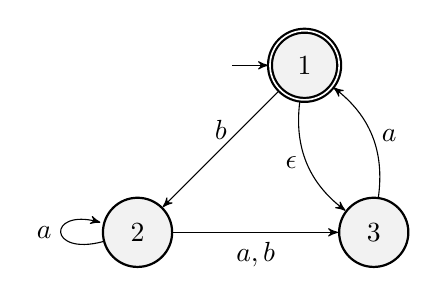
\begin{tikzpicture}
\node[state, initial, accepting] (1) {$1$};
\node[state, below left of=1] (2) {$2$};
\node[state, right of=2] (3) {$3$};
\draw (1) edge[above] node{$b$} (2)
(1) edge[below, bend right, left=0.3] node{$\epsilon$} (3)
(2) edge[loop left] node{$a$} (2)
(2) edge[below] node{$a, b$} (3)
(3) edge[above, bend right, right=0.3] node{$a$} (1);
\end{tikzpicture}

\caption{Caption of the FSM2}
\label{fig:my_label2}
\end{figure}


\bigskip

\begin{figure}[ht] % 'ht' tells LaTeX to place the figure 'here' or at the top of the page
\centering % centers the figure

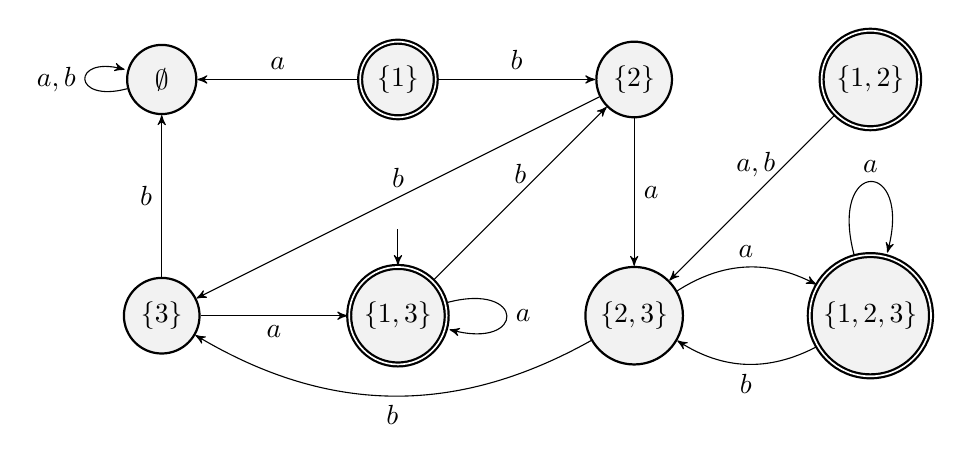
\begin{tikzpicture}
\node[state] (phi) {$\emptyset$};
\node[state, accepting, right of=phi] (1) {$\{1\}$};
\node[state, right of=1] (2) {$\{2\}$};
\node[state, accepting, right of=2] (12) {$\{1, 2\}$};
\node[state, below of=phi] (3) {$\{3\}$};
\node[state, initial, initial where=above, accepting, right of=3] (13) {$\{1, 3\}$};
\node[state, right of=13] (23) {$\{2, 3\}$};
\node[state, accepting, right of=23] (123) {$\{1, 2, 3\}$};
\draw (phi) edge[loop left] node{$a, b$} (phi)
(1) edge[above] node{$a$} (phi)
(1) edge[above] node{$b$} (2)
(2) edge[right] node{$a$} (23)
(2) edge[above] node{$b$} (3)
(12) edge[above, pos=.3, left=2pt] node{$a, b$} (23)
(3) edge[left] node{$b$} (phi)
(3) edge[below] node{$a$} (13)
(13) edge[loop right] node{$a$} (13)
(13) edge[above] node{$b$} (2)
(23) edge[bend left, above] node{$a$} (123)
(23) edge[bend left, below] node{$b$} (3)
(123) edge[loop above] node{$a$} (123)
(123) edge[bend left, below] node{$b$} (23);
\end{tikzpicture}

\caption{Caption of the FSM3}
\label{fig:my_label3}
\end{figure}



\end{document}